% This file was converted to LaTeX by Writer2LaTeX ver. 1.2
% see http://writer2latex.sourceforge.net for more info
\documentclass[11pt]{article}
\usepackage[utf8]{inputenc}
\usepackage[T1]{fontenc}
\usepackage[spanish,english]{babel}
\usepackage{amsmath}
\usepackage{amssymb,amsfonts,textcomp}
\usepackage{array}
\usepackage{supertabular}
\usepackage{hhline}
\usepackage{graphicx}
\makeatletter
\newcommand\arraybslash{\let\\\@arraycr}
\makeatother
\setlength\tabcolsep{1mm}
\renewcommand\arraystretch{1.3}
\newcounter{Figura}
\renewcommand\theFigura{\arabic{Figura}}
\title{}
\begin{document}
  
   \begin{titlepage}

\begin{center}
\vspace*{-1in}

FACULTAD DE INGENIERIA\\
\vspace*{0.15in}
UNIVERSIDAD DE LA REPUBLICA \\
\vspace*{0.6in}
\vspace*{0.2in}
\begin{Large}
\textbf{Diseño} \\
\end{Large}
\vspace*{0.3in}
\end{center}

\begin{minipage}{0.4\textwidth}
\begin{flushleft} \large
\emph{Autor:}\\
Julio Saráchaga\\
\bigskip
\emph{Contraparte del cliente:}\\
Ing. Fernanda Molina
\end{flushleft}
\end{minipage}
\begin{minipage}{0.4\textwidth}
\begin{flushright} \large
\emph{Supervisor:} \\
Dr. Gustavo Betarte\\
\bigskip
\emph{Supervisor alterno:} \\
Ing. Marcelo Rodríguez
\end{flushright}
\end{minipage}\\[3cm]

\end{titlepage}

\clearpage\setcounter{page}{1}\section[Introducción]{Introducción}
\foreignlanguage{spanish}{Durante el análisis, se identificaron los requerimientos del sistema. Se pretende que en este
capitulo se proponga una solución que respete los requerimientos que se determinaron.}

\foreignlanguage{spanish}{En el capitulo se describe el funcionamiento de la herramienta propuesta identificando los
componentes que participan en dicho proceso. Se detalla el modelo de datos creado para la base de datos. Se explica la
arquitectura de la aplicación con la función de cada una de sus componentes.}

\section[Contexto para el uso del sistema]{\foreignlanguage{spanish}{Contexto para el uso del sistema}}
\foreignlanguage{spanish}{Por medio del sistema propuesto es posible ingresar información de seguridad, correlacionarla
con información existente en el sistema y luego de ser sanitizada, compartirla con organizaciones socias.}


\bigskip

\foreignlanguage{spanish}{El sistema ha sido diseñado para que sea utilizado por grupos de seguridad. Se busca que
dichos grupos puedan compartir información de incidentes de seguridad representada con el lenguaje STIX y que sea
distribuida utilizando TAXII. El diseño y desarrollo de STIX y TAXII ha sido realizado por MITRE con el apoyo de la
comunidad. El intercambio de información da a las organizaciones la posibilidad de identificar adecuadamente las
amenazas dando evidencias específicas de su existencia.}

%
%Ver como se puede exapndir esto.
%Agregar con algo sacado del estado del arte.
%Ver si esto se puede extender
%Encontrar que poner
%
%April 21, 2014 7:43 PM


\section[Componentes del sistema]{\foreignlanguage{spanish}{Componentes del sistema}}

\bigskip

\foreignlanguage{spanish}{En esta sección se presenta el sistema diseñado, en la figura 1 se muestra su arquitectura. El
sistema busca darle a las organizaciones la capacidad de intercambiar información de seguridad de forma automática y
segura}%
%Ver como se puede exapndir esto.
%Agregar con algo sacado del estado del arte.
%Ver si esto se puede extender
%Encontrar que poner
%
%April 21, 2014 7:43 PM
\foreignlanguage{spanish}{. Se busca integrar a RTIR dicha capacidad utilizando las herramientas mencionadas
anteriormente. Para ello se busca extender RTIR para poder consumir servicios web publicados por la aplicación TAXII,
además se puede utilizar la API Rest de RTIR para realizar el manejo de las estructuras utilizadas por éste. El sistema
TAXII es un desarrollo nuevo que utiliza librerías provistas por MITRE, estas son utilizadas para representar e
intercambiar la información.}


\bigskip

 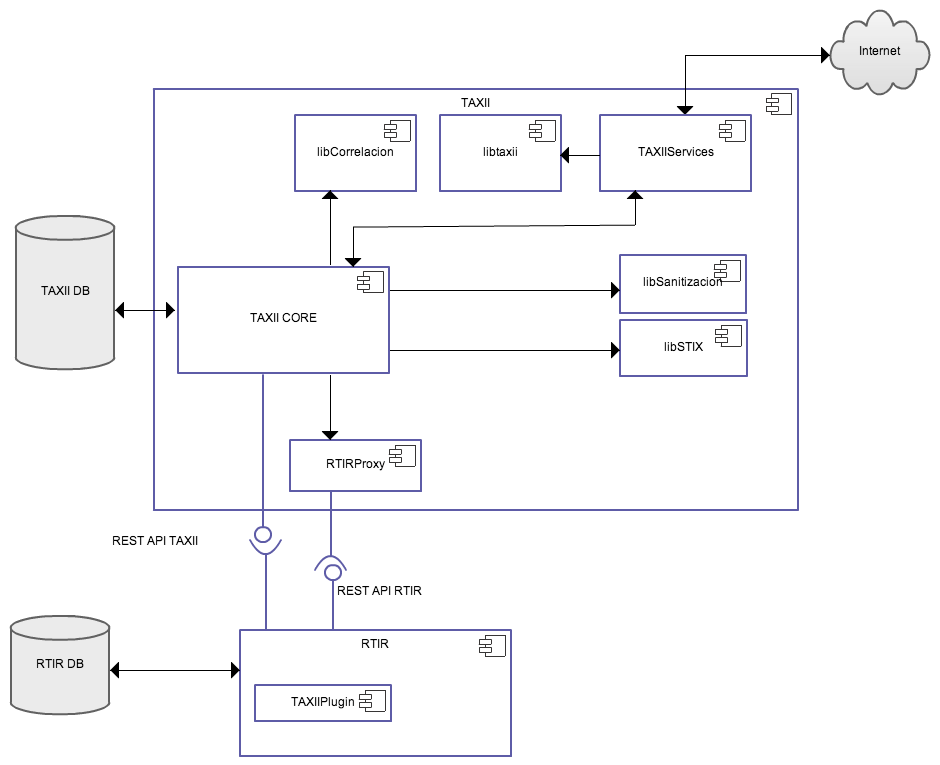
\includegraphics[width=5.7638in,height=4.6909in]{Diseno-img003.png} 

{\centering\bfseries
\foreignlanguage{spanish}{Figura }\stepcounter{Figura}{\theFigura}\foreignlanguage{spanish}{ - Arquitectura del sistema}
\par}


\bigskip

\section[Aspectos generales de las componentes del sistema]{\foreignlanguage{spanish}{Aspectos generales de las
componentes del sistema}}
\foreignlanguage{spanish}{La aplicación RTIR recibe datos ingresados por un analista y los transmite a la aplicación
TAXII. Para realizar dicha transmisión es necesario extender RTIR por medio de
}\foreignlanguage{spanish}{\textit{plugins}}\foreignlanguage{spanish}{ para consumir una API REST publicada por el
cliente TAXII.}

\foreignlanguage{spanish}{La aplicación RTIR también puede recibir de la aplicación TAXII información, dicha información
puede estar relacionada a tickets existentes y contener soluciones a problemas, identificación de atacantes, etc.}


\bigskip

\foreignlanguage{spanish}{La aplicación TAXII recibe datos de RTIR así como también de organizaciones socias, en un
futuro se podría dar la posibilidad de que la aplicación TAXII recibiera datos de sensores que se encuentren en la red
de la organización. Luego de que los datos son recibidos y almacenados se correlacionan con los ya existentes. De la
correlación se pueden obtener soluciones a problemas encontrados, información sobre ataques realizados, identificación
de atacantes, etc. En caso de que exista información de utilidad se pueden ingresar notas a tickets o relacionar
tickets existentes en el RTIR.}

\foreignlanguage{spanish}{También se podría compartir información con otras organizaciones para colaborar en la lucha
contra amenazas. Para realizar dicho intercambio se representa la información utilizando STIX y luego se intercambia
utilizando TAXII. Se utilizan librerías provistas por MITRE para realizar la representación y el intercambio de la
información.}


\bigskip

\foreignlanguage{spanish}{Se pueden identificar claramente dos aplicaciones en el sistema las cuales son independientes,
dichas aplicaciones son RTIR y TAXII. La aplicación TAXII es independiente de la aplicación RTIR. Siendo posible
reemplazar esta última por otra herramienta con funcionalidades similares.}

\subsection[RTIR]{\foreignlanguage{spanish}{RTIR}}
\foreignlanguage{spanish}{Esta componente presenta las funcionalidades originales de la herramienta RTIR con un agregado
específico implementado para este proyecto. RTIR es la componente de la aplicación encargada de realizar el manejo de
los incidentes.}

\foreignlanguage{spanish}{Se agrega un plugin que permite invocar una API REST en la aplicación TAXII. \ }

%
%Ver como se puede exapndir esto.
%Agregar con algo sacado del estado del arte.
%Ver si esto se puede extender
%Encontrar que poner
%
%April 21, 2014 7:43 PM
\foreignlanguage{spanish}{La base de datos de la aplicación es RTIR DB y es únicamente utilizada por la componente RTIR,
no hay acceso desde ningún otro componente a ella. Además es importante destacar que la base de datos de RTIR no se
modifica de ningún modo.}


\bigskip

\subsection[TAXII\ \ ]{\foreignlanguage{spanish}{TAXII\ \ }}

\bigskip

\foreignlanguage{spanish}{La segunda componente presente es TAXII, está compuesta por otros componentes implementados
durante el proyecto así como por librerías provistas por MITRE. Los componentes provistos por MITRE son libTAXII y
libSTIX, a estos no se le realizaran cambios. El componente TAXII utiliza los componentes TAXIICore, RTIRProxy y
TAXIIServices, estos son implementados durante el transcurso del proyecto. Los componentes libSanitizacion y
libCorrelacion si bien son implementados podrían valerse de librerías ya existentes para realizar la correlación y la
sanitización de los datos.}


\bigskip

\subsection[libTAXII]{\foreignlanguage{spanish}{libTAXII}}

\bigskip

\foreignlanguage{spanish}{Es una librería que provee una representación de objetos de los mensajes TAXII, cuenta además
con una serie de métodos para el manejo de dichos mensajes. Provee clientes para http y https. La librería se utiliza
para generar los mensajes y dispone métodos para transformarlos a xml, estos xml son utilizados en los intercambios
entre cliente y servidor.}

\subsection[libSTIX]{\foreignlanguage{spanish}{libSTIX}}
\foreignlanguage{spanish}{libSTIX es una librería provista por MITRE para parsear, manipular y generar contenido STIX.}

\subsection[RTIRProxy]{\foreignlanguage{spanish}{RTIRProxy}}
\foreignlanguage{spanish}{RTIRProxy es la componente encargada de integrarse con RTIR, para ello consume la API REST
provista por RTIR para el manejo de tickets. Por ser una API REST la comunicación está encapsulada en el protocolo
http. La razón de la existencia de esta componente es facilitar el uso de otros sistemas en lugar de RTIR. Lo que se
logra es que si otro sistema tiene una API o un método de integración distinto al de RTIR se re implemente esta
componente. La única premisa que se debe cumplir es que la interfaz con la cual se comunique TAXIICore se mantenga.
Dentro de dichos tipos de integración podría encontrarse otra API REST o web services con SOAP. }

\subsection[TAXIICore]{\foreignlanguage{spanish}{TAXIICore}}
\foreignlanguage{spanish}{Es la componente encargada de agendar la correlación de datos, dicha correlación es realizada
con información almacenada en TAXII DB y se realiza por medio de la componente libCorrelación. }

\foreignlanguage{spanish}{Es necesario que este componente tenga una interfaz de web services REST para realizar la
comunicación con el RTIR. En dicha interfaz se deben dar operaciones para realizar el alta de información, obtener
información de servicios publicados por contrapartes, enviar y recibir información de seguridad entre contrapartes.}

\foreignlanguage{spanish}{Además debe proveer una interfaz para que la componente TAXIIServices envíe la información
recibida en la aplicación TAXII, en dicha interfaz se deben recibir tanto paquetes STIX así como información de los
intercambios realizados con TAXII. }

\foreignlanguage{spanish}{La información tomada de la base de datos es enviada en forma de objetos STIX junto a las
políticas definidas por los administradores para que sea sanitizada. }\foreignlanguage{spanish}{Luego de que la
información es sanitizada es enviada a TAXIIServices para que sea compartida con las organizaciones socias.}

\subsection[libSanitizacion]{\foreignlanguage{spanish}{libSanitizacion}}
\foreignlanguage{spanish}{Esta es la componente encargada de realizar la sanitización de la información que se desea
intercambiar entre los sistemas. En }\foreignlanguage{spanish}{[JBH04] se plantea un modelo donde se realiza
sanitización de información representada por medio de IDMEF. En dicho paper se modifican los mensajes IDMEF utilizando
XSLT (Extensible Stylesheet Language Transformations). Se busca tener una implementación que realice XSLT para
documentos STIX. La componente se alimenta de políticas definidas por los administradores para realizar la
sanitización.}

\subsection[libCorrelacion]{\foreignlanguage{spanish}{libCorrelacion}}
\foreignlanguage{spanish}{Es la componente encargada de la correlación de los datos del sistema.}%
%Ver como se puede exapndir esto.
%Agregar con algo sacado del estado del arte.
%Ver si esto se puede extender
%Encontrar que poner
%
%April 21, 2014 7:43 PM
\foreignlanguage{spanish}{ La componente ayuda a agrupar datos que tengan características similares lo que facilita el
trabajo de los administradores y de más valor a la información recibida. Se pueden pensar distintos métodos para
realizar las correlaciones y de ahí se desprende la necesidad que sea un componente separado del Core del sistema.}

\subsection[TAXIIServices]{\foreignlanguage{spanish}{TAXIIServices}}
\foreignlanguage{spanish}{Esta componente es una implementación de los servicios TAXII como se especifica en
}\foreignlanguage{spanish}{[M13] \ y \ [M14]. }

\foreignlanguage{spanish}{TAXIIServices provee los siguientes servicios:}

\liststyleWWNumi
\begin{itemize}
\item \foreignlanguage{spanish}{Inbox: Por medio de este servicio el sistema acepta mensajes enviados por un productor
en intercambios iniciados por este. }
\item \foreignlanguage{spanish}{Poll: Este servicio es el que utiliza el sistema para consumir datos provenientes de un
TAXII Data Feed en un productor.}
\item \foreignlanguage{spanish}{Discovery: Es el servicio encargado de la comunicación de información referente a la
disponibilidad y uso de los servicios TAXII en el sistema.}
\end{itemize}
\foreignlanguage{spanish}{Utiliza la componente libTAXII para crear mensajes TAXII y de esa forma realizar el
intercambio de documentos STIX recibidos de libSanitizacion. Los mensajes que son recibidos de otros socios son pasados
a la componente TAXIICore para que sea almacenada y luego correlacionada con datos existentes. }


\bigskip


\bigskip

\section[Comunicación entre los componentes]{\foreignlanguage{spanish}{Comunicación entre los componentes}}

\bigskip

\foreignlanguage{spanish}{En la comunicación entre RTIR y la aplicación TAXII se utiliza REST (Representational State
Transfer), en este tipo de servicio web se trata de emular \ el protocolo http o algún protocolo similar usando la
restricción de proveer una interfaz a un conjunto conocido de operaciones estándar (GET, PUT, etc). Se utiliza este
tipo de servicio web debido a que RTIR provee una API de este tipo. }


\bigskip

\foreignlanguage{spanish}{El intercambio entre las distintas organizaciones se realiza por medio de HTTP/HTTPS. Esto se
debe a que hasta el momento MITRE solo ha especificado el intercambio por medio de dicho protocolo. Se podrían utilizar
otros protocolos para realizar el intercambio pero sería necesario que MITRE definiera las especificaciones para su
uso, un ejemplo de ellos podría ser SOAP.}


\bigskip

\section[Modelo de datos]{\foreignlanguage{spanish}{Modelo de datos}}
\foreignlanguage{spanish}{El modelo de datos diseñado se adapta a las necesidades de TAXII, dichas necesidades están
definidas en \ [M15], además se agrega una tabla para realizar el mapeo entre los elementos del RTIR y los elementos
TAXII intercambiados.}

\foreignlanguage{spanish}{En la figura 2 se ve el modelo de datos \ y a continuación se explica cada una de sus
componentes.}

 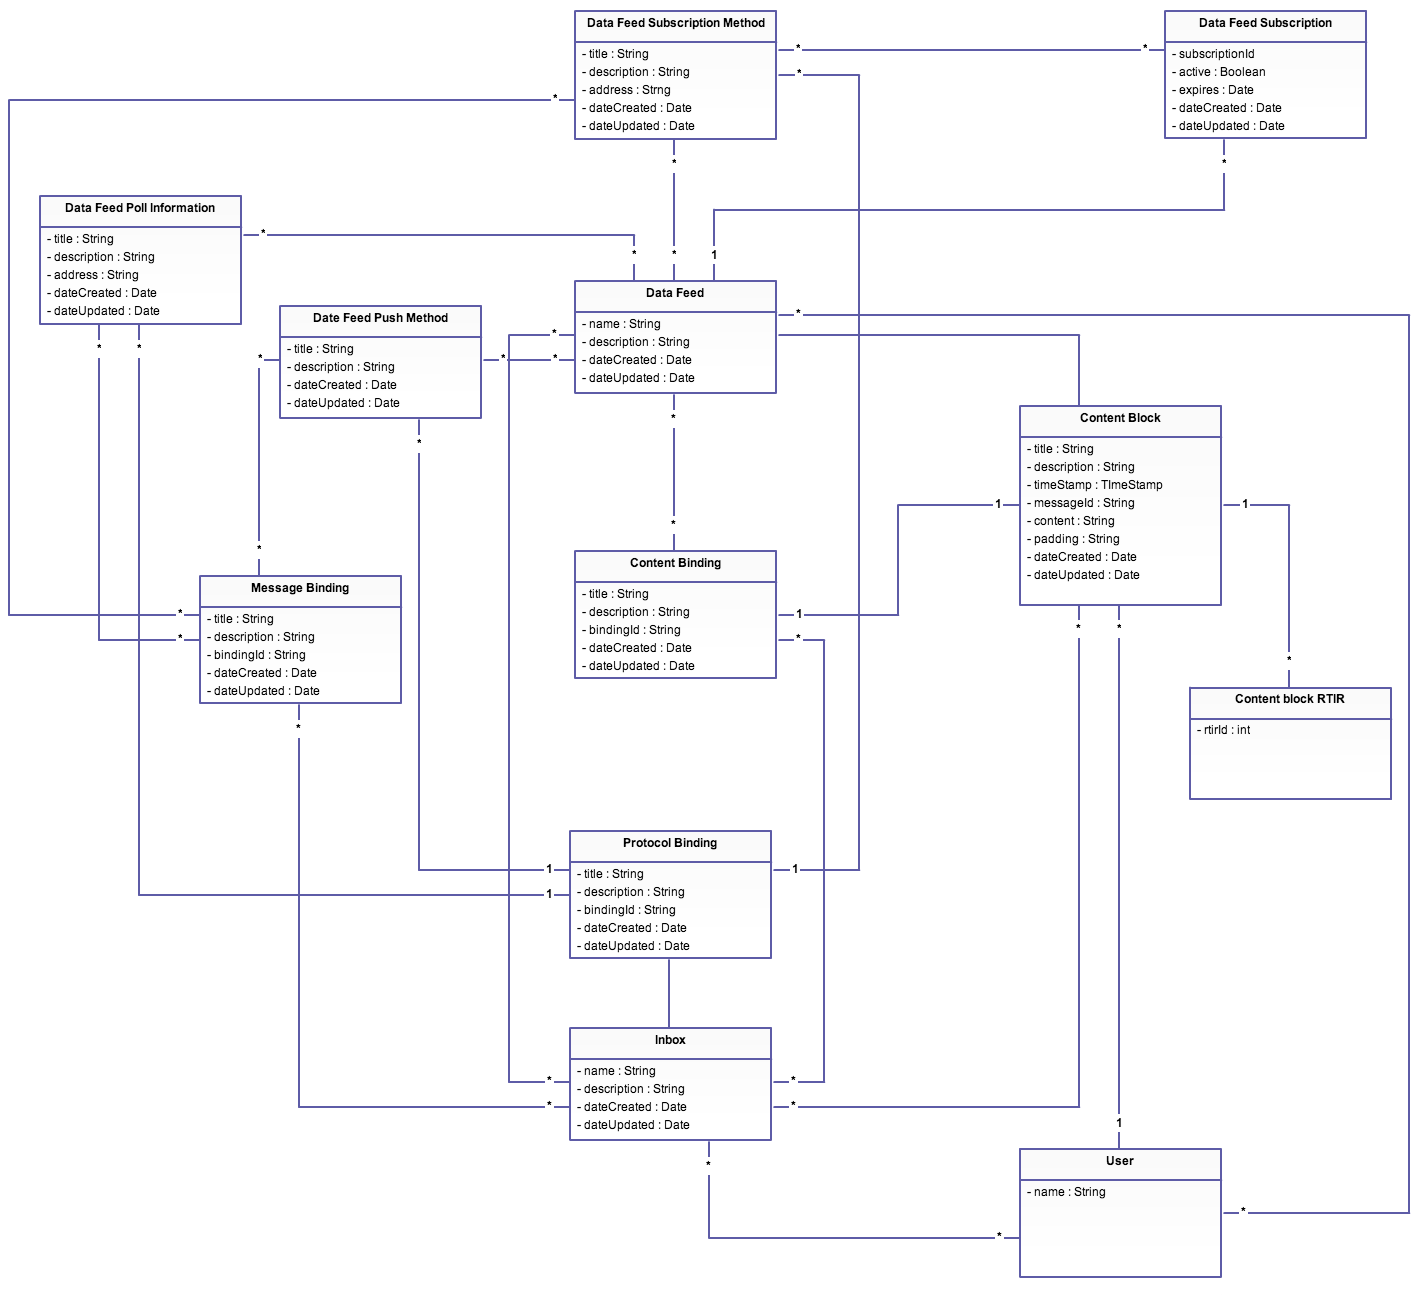
\includegraphics[width=5.7638in,height=5.3126in]{Diseno-img004.png} 


\bigskip


\bigskip


\bigskip

\liststyleWWNumii
\begin{itemize}
\item \foreignlanguage{spanish}{Protocol Binding: Es un elemento utilizado para establecer el protocolo de intercambio
soportado por una implementación de TAXII.}
\item \foreignlanguage{spanish}{Content Binding: Es utilizado para establecer el tipo de contenido soportado para un
cierto intercambio realizado con TAXII, por ejemplo:
}\foreignlanguage{spanish}{\textit{Poll}}\foreignlanguage{spanish}{,
}\foreignlanguage{spanish}{\textit{Inbox}}\foreignlanguage{spanish}{, etc.}
\item \foreignlanguage{spanish}{Message Binding: Es utilizado para establecer el tipo de sintaxis para un intercambio
realizado con TAXII.}
\item \foreignlanguage{spanish}{Data Feed Push Method: Es utilizado para establecer los protocolos que pueden ser
utilizados para enviar contenido por medio de una subscripción. Esto se utiliza en un mensaje de
}\foreignlanguage{spanish}{\textit{tipo Feed Information Response}}\foreignlanguage{spanish}{. Es definido en [M14].}
\item \foreignlanguage{spanish}{Data Feed Poll Information: Tiene la finalidad de establecer los protocolos soportados y
las direcciones de una fuente de información (}\foreignlanguage{spanish}{\textit{Data
Feeds}}\foreignlanguage{spanish}{). Es utilizado en los mensajes de }\foreignlanguage{spanish}{\textit{Feed Information
Response}}\foreignlanguage{spanish}{ como se define en [M14].}
\item \foreignlanguage{spanish}{Data Feed Subscription Method: Es utilizado para identificar el protocolo y la dirección
de un servicio de }\foreignlanguage{spanish}{\textit{Feed Managment}}\foreignlanguage{spanish}{ que pueda procesar las
subscripciones a fuentes de información TAXII.}
\item \foreignlanguage{spanish}{Content Block: Representa el contenido de los mensajes
}\foreignlanguage{spanish}{\textit{Poll Response }}\foreignlanguage{spanish}{o }\foreignlanguage{spanish}{\textit{Inbox
Messages}}\foreignlanguage{spanish}{. Es necesario señalar que el campo
}\foreignlanguage{spanish}{\textit{content}}\foreignlanguage{spanish}{ representa un mensaje STIX. Dicho mensaje
representa la información de seguridad estructurada la cual fue representada utilizando el lenguaje STIX.}
\item \foreignlanguage{spanish}{Data Feed: Representa una fuente de información TAXII, los usuarios se suscriben a
dichas fuentes de información para recibir datos que sean de su interés. }
\item \foreignlanguage{spanish}{Data Feed Subscription: Representa una subscripción a fuentes de datos TAXII.}
\item \foreignlanguage{spanish}{Inbox: Representa un }\foreignlanguage{spanish}{\textit{inbox
}}\foreignlanguage{spanish}{TAXII, estos son el mecanismo por el cual los consumidores reciben información de los
productores de información. La representación permite que un
}\foreignlanguage{spanish}{\textit{inbox}}\foreignlanguage{spanish}{ este asociado a ningún o muchas fuentes de datos.
}
\item \foreignlanguage{spanish}{Content Block RTIR: Representa el nexo entre los contenidos TAXII y los tickets
existentes en RTIR.}
\end{itemize}

\bigskip


\bigskip


\bigskip


\bigskip
\newpage
\foreignlanguage{spanish}{\ [JBH04] Marko Jahnke, Michael Bussmann, Sven Henkel, ``Components for Cooperative Intrusion
Detection in Dynamic Coalition Enviroments'', RTO IST Symposium on Adaptive Defence in Unclassified Networks, 2004}


\bigskip

\foreignlanguage{spanish}{[M14] Mitre Corporation, ``The TAXII Services Specification'', 2014}


\bigskip

\foreignlanguage{spanish}{[M13] Mitre Corporation, ``The TAXII HTTP Protocol Binding Specification'', 2013}


\bigskip

\foreignlanguage{spanish}{[M12] Mitre Corporation, ``}TAXII HTTP Protocol Binding Specification'', 2013


\bigskip

\foreignlanguage{spanish}{[M15] Mitre Corporation, ``The TAXII XML Message Binding Specification'', 2013}


\bigskip
\end{document}
